\documentclass[12pt]{article}

\usepackage{latex/ediArticle}  %from ediArticle.sty
%\usepackage{multirow}
\usepackage{amsmath}
%\usepackage{amssymb}
%\usepackage[normalem]{ulem}
%\usepackage[table]{xcolor}


%%%%%%%%%%%%%%%%%%%%%%%%%%%%%%%%%%%%%%%%%%%%%%%%%%%%%%
\title{\LARGE \bfseries \vspace{-2cm} Burden and health-related quality of life among caregivers of people with motor neuron disease}
\author{\vspace{-2cm}}
\date{\vspace{-2cm}}

\begin{document}

% Set font size to 13pt
\fontsize{13pt}{15pt}\selectfont

\maketitle


%%%%%%%%%%%%%%%%%%%%%%%%%%%%%%%%%%%%%%%%%%%%%%%%%%%%%%
\section{Introduction}
Motor neuron disease (MND) is a progressive neurodegenerative disease that impacts not only patients but also their informal caregivers. Several studies on ALS in Australia \parencite{lillo_caregiver_2012}, United States \parencite{qutub_life_2014, burke_caregiver_2015, roach_dynamics_2009}, Turkey \parencite{tulek_care_2023}, Ireland \parencite{galvin_caregiving_2016}, Germany \parencite{schischlevskij_informal_2021}, and China \parencite{geng_patients_2017}, have investigated the factors contributing to caregiver burden in ALS and the associated impact of caregiving on the quality of life of these individuals. \textcite{lillo_caregiver_2012} found that patients' abnormal behavior and caregiver stress were the strongest predictors of high caregiver burden, while physical disability was not significantly associated. 

A cross-sectional study of 33 patient-caregiver pairs, which showed that high caregiver burden was associated with greater patient apathy, disinhibition, and executive dysfunction, as well as caregiver distress \parencite{burke_caregiver_2015}. \textcite{qutub_life_2014} study also found that patients' functional status did not affect caregivers' burden. \textcite{schischlevskij_informal_2021} results showed that caregiver burden increased with patients' decline in functional status - patients' wheelchair use and need for supervision were the strongest predictors of burden.

\textcite{tulek_care_2023} study corroborates sex as having a significant relationship to caregivers' burden. \textcite{geng_patients_2017} found an association between caregiver burden and older caregiver age. Other factors related to caregivers' burden are difficulties in managing ALS, the emotional or psychosocial impact of caregiving, limitations or restrictions, and the effects on relationships that caregiving has on the caregivers \parencite{galvin_caregiving_2016}. Patients' functional status affect caregiver quality of life \parencite{roach_dynamics_2009}.

%%%%%%%%%%%%%%%%%%%%%%%%%%%%%%%%%%%%%%%%%%%%%%%%%%%%%%
\section{Methods}

\subsection{Study design and participants}
COMMEND was a XXX designed to YYY. The study design, patient
characteristics, and baseline costs and resource-use data
have been reported \parencite{gould_randomised_2022}. The present study focuses on the caregivers; the baseline characteristics and quality of life have been reported previously for patient  \parencite{gould_acceptance_2024}. Patients with
probable/confirmed?? MND, CRITERIA???, were enrolled between
DATE and DATE, mostly at WHERE. Patients were
also required??? to have a primary caregiver who was
willing to participate in the study. Caregivers were included if BRIEF INCLUSION CRITERIA [cite trial]. 

\subsection{Data and questionnaires}
Data were collected for patients and caregivers at the
baseline visit and at baseline, 6 months, and 18 months during WHICH?? visits. Full details of the baseline patient and caregiver
demographics and characteristics, including comorbidities
and medications used, have been reported previously \parencite{gould_acceptance_2024, keetharuth_costeffectiveness_2024}.

% Paraphrase this
We assessed caregiver burden at every visit using the 22-item version of Zarit Burden Interview (ZBI). ZBI is a widely-used instrument for assessing the perceived burden experienced by caregivers \parencite{zarit_relatives_1980}. The questions cover the caregiver’s health, psychological well-being, finances, social life, and relationship with the patient. The 22-item version of ZBI contains five-point Likert-style questions with responses to each item ranging from 0, denoting “never”, to 4, denoting “nearly always”. \parencite{zarit_hidden_1985}. The total score therefore ranges from 0 to 88, with a higher score indicating a greater perceived care burden. 

% Paraphrase this and shorten
Caregivers self-assessed their HRQoL at using the EuroQol Visual Analogue Scale (EQ-VAS) and 5-dimension (EQ-5D) questionnaires [\textbf{REF}]. For EQ-5D, they scored their current health state in each of five domains (pain/discomfort, anxiety/depression, mobility, usual activities, and self-care) using a 3-point scale (no, moderate, or extreme problems). From the health-state profile obtained, a scoring algorithm using English preference weights [\textbf{REF}] was used to calculate a total utility score (EQ-5D index score) between 0 (represents death) and 1.0 (represents perfect health). Caregivers rated their current health status on the day of assessment using EQ-VAS, which ranges from 0 (worst imaginable health) to 100 (best possible health). The mean norm value in the English population is reportedly XX (\textbf{REF}). 

Factors related to the informal caregivers (\autoref{tab_var_category}), that is age,sex, educational level, work status, change in work status, relation to the patient with ALS, and whether cohabiting with the patient, was collected with the study‐specific questionnaire. It also included questions on time spent on informal caregiving in personal ADL (P‐ADL),that is feeding, bathing, dressing, toileting and transfer; instrumental ADL (I‐ADL), that is cooking, transport, cleaning and shopping; andother activities that the patient with ALS used to do before disease onset. The first set of variables were caregiver sociodemographic characteristics.  such as sex (DEFINE), age (DEFINE), level of education (DEFINE), employment status (DEFINE). We also asked respondents if they had any medical conditions. Other variables were caregiving context, including relationship with care recipient (DEFINE), intensity of caregiving activities (DEFINE), and how long has been looking after (DEFINE).

We also collected information on characteristics of patients with ALS (\autoref{tab_var_category}). These included age, sex, marital status, employment situation, educational level, presence and number of comorbidities, duration of disease, disease severity. These were collected during XXX \parencite{gould_acceptance_2024}. Disease severity was measured using the ALS Functioning Rating Scale‐Revised, ALSFRS‐R \parencite{cedarbaum_alsfrs-r_1999}. We used the algorithm developed by \textcite{balendra_estimating_2014} to calculate King's clinical stages from ALSFRS-R scores. The King's staging system is based on disease burden and consists of five disease stages (1 to 5) with stage 1 being onset of disease in one anatomical region and stage 5 being death.

\hspace{1em}
\begin{table}[H]
    \centering \singlespacing \small
    \caption{Categorization of independent variables}
    \begin{tabular}{|L{6cm}|L{9cm}|}
        \hline
        \PlainInput{tables/tab_var_category}
    \end{tabular}
    \label{tab_var_category}
    \caption*{\footnotesize \textit{Notes:} Donec sit amet viverra justo}
\end{table}


\subsection{Statistical analysis}
We described the characteristics of the participants (patients with MND and caregivers) using means and standard deviations for continuous variables and using numbers and percentages for categorical variables. We used univariate linear regression to examine the direction and size of the relationships between caregiver burden and possible influencing factors on  caregivers’ burden (ZBI) and health-related quality of life (EQ-5D). We then conducted a multiple regression analysis to test the extent to which these variables explained ZBI and EQ-5D. We selected variables to add to multiple linear regression by adopting a critical level of significance (p $\leq$ 0.10) in the univariate analysis.
%Spearman correlation coefficients examined the within- subject associations between continuous variables such as caregiver ZBI total scores, EQ-5D index scores, EQ-5D VAS scores, and T-IADL, at baseline, at 18 months, and for the change from baseline to 18 months. We inter- preted correlation coefficients of 0–0.19 as very weak and 0.20–0.39 as weak.
All analysis were conducted using Stata version 18.0 (StataCorp, College Station, Texas, USA).

\section{Results}
%At baseline, the study cohort analyzed comprised 1495 patients with mild AD dementia (n = 566), moderate AD dementia (n = 472), or MS/S AD dementia (n = 457), and their caregivers (n = 1495). The number of caregivers and patients from each country was as follows: France, n = 419; Germany, n=550; UK, n=526. A total of 1040 caregivers attended the 18-month visit (69.6\%). The main reasons for discontinuation from the study were patient institutionalization (n = 214), the patient had died (n = 92), the caregiver/patient had decided to leave the study (n =119), or the caregiver/patient was lost to follow-up (n = 26). The number of caregivers with available data at the 18-month visit was: ZBI, n = 932; EQ-5D, n = 934; T- IADL, n = 983. The number of caregivers with available data for the change from baseline to 18 months was: ZBI, n = 931; EQ-5D, n = 933; and T-IADL, n = 982.

%From all over Germany, out of 404 returned questionnaires, 325 patients with ALS, cor- responding to the inclusion criteria, were identified. Additionally, patients without a filled caregiver questionnaire were excluded from further analyses, resulting in 249 full datasets that were analyzed, including questionnaires completely answered by ALS patients and their main CGs. Data from both the patient’s and CG’s perspectives were evaluated and presented in this study. Related to the estimated prevalence of ALS [66] in Germany, about 6600 patients may have lived with this diagnosis in 2019 [67]. Overall, we managed to include nearly 4\% of them and their CGs for this study. The distribution of our patients roughly matched the population distribution by state in Germany, although patients from Lower Saxony were overrepresented (the study’s principal investigator was located at Hannover), and some states were underrepresented (Appendix A Table A1).

\subsection{Caregiver and patient characteristics}
%The baseline sociodemographic and clinical characteristics of the caregivers and patients are summarized in Table 1. Caregivers had a mean (SD) age of 67.3 (12.0) years and most were female (64.2%), the spouse of the patient (65.9%), and living with the patient (76.0%). The majority of caregivers reported medical conditions (58.6%; mean of 1.1 medical conditions), most commonly hypertension (36.8%), hypercholesterolemia (23.5%), and depression (10.1%). Approximately one-quarter of the caregivers (23.8%) reported working for pay. The patients had a mean (SD) age of 77.6 (7.7) years, 54.8% were female, mean (SD) time since diagnosis was 2.2 (2.2) years, and 73.6% had comorbidities (mean of 1.4 comorbidities). ZBI total scores at baseline ranged from 0 to 80 and the mean (SD) score was 29.0 (15.1). 

%Of the patients in this study, 64.1% were male, which matches previous findings that ALS is more prevalent in men [68]. The median age was 65 with a range from 27 to 88 years old. In general, the distribution of gender and age in our cohort appeared to be representative according to previous literature [69,70]. Most patients (89.3%) were married or in a partnership, and lived together with their partner (91.0%). About half of the patients (48.2%) used a wheelchair, 21.3% used home ventilator support, 15.3% were nourished using a percutaneous endoscopic gastrostomy (PEG), and 41.6% of patients required permanent (24 h) supervision. The median BI score was 60/100 and the median ALSFRS-R score was 32.5/48. No significant differences between men and women were observed, besides that female patients in our cohort showed a stronger impaired functional status (mean BI = 50.97/100, SD = 31.26, n = 88/mean ALSFRS-R = 29.61/48, SD = 9.33, n = 87) than men (mean BI = 62.58/100, SD = 30.79, n = 157/mean ALSFRS-R = 32.38/48, SD = 9.50, n = 157; BI, U = 5415.00; Z = 2.81; p = 0.005; n = 245/ALSFRS-R, U = 5593.00; Z = 2.34; p = 0.019; n = 244). The BI groups and the King’s Stages were well distributed, as the cohort included patients in all disease severity stages (Table 1).

%In the study, 69.9\% of the CGs were female. The median age was 61 with a range from 18 to 88 years old. In our cohort, female CGs were younger than male CGs (U = 4693.00; Z = 3.46; p = 0.001; n = 248). Out of four possible patterns, in 61.2\% the patient was male and the CG was female, in 26.9\% the patient was female and the CG was male, in 9.0\% the patient and the CG were female, and in 2.9\% of the cases, the patient, as well as the CG were male. Most CGs (83.1\%) were the patients’ spouses with whom they lived together, which reflects previous studies [6,27]. All but 0.8\% (friends, n = 2) of the CGs were direct family members. While 8.0\% had to stop working due to their partner’s condition and 47.8\% were either retired, unemployed or a homemaker, 44.2\% of the CGs were still emplo=yed and thus worthy of consideration for the work life impairment analysis. The median duration of caregiving (DOC) was three hours per day (as stated by the main CG; additional hours by more than one CG per patient are possible). 42.6\% of the CGs reported an individual health deterioration due to caregiving. With a median ZBI score of 26/88, the cohort was highly burdened [59]. The EQ-VAS median with 75/100 was lower than the calculated EQ-5D-5L index value median with 0.909/1. The median HADS-D and HADS-A scores were 8/21 and 9/21, respectively, which indicated the presence of depression and anxiety. Besides higher anxiety in female CGs (see Section 3.6), no mentionable differences between men and women were observed (Table 2).

Descriptive statistics in (\autoref{tab_desc_stat}). 

\hspace{1em}
\begin{table}[H]
    \centering \singlespacing \small
    \caption{Descriptive statistics.}
    \begin{tabular}{|L{5cm}|R{3.2cm}|}
        \hline
        \PlainInput{tables/tab_desc_stat}
    \end{tabular}
    \label{tab_desc_stat}
    \caption*{\footnotesize \textit{Notes:} Data are based on participants with non-missing baseline caregiver burden and quality of life data. n, number; SD, standard deviation.
}
\end{table}

\subsection{Caregiver burden in relation to patient's functional status}

%The ANOVA showed statistically significant differences in the arithmetic means of the ZBI scores between the BI groups (Figure 1a) and the King’s Stages (Figure 1b). This means that an increase in patient’s functional impairment led to a higher caregiver burden. This result was supported by a positive correlation between the ZBI score and the King’s Stages (rs = 0.300, p < 0.001, n = 237) and a negative correlation between the ZBI score and the ALSFRS-R (rp = −0.460, p < 0.001, n = 237). Additionally, there was a strong negative correlation between the ZBI score and the BI score (rp = −0.555, p < 0.001, n = 242).

%The mean (SD) ZBI total score showed a greater burden for the patient groups with worse disease severity: 24.6 (14.2), 29.4 (14.8), and 34.1 (14.8) for the mild, moderate, and MS/S AD dementia groups, respectively (ANOVA P < 0.001) (Table 2). The mean (SD) change in ZBI total score from baseline to 18 months was 4.9 (12.6) for the overall cohort of caregivers, and differed significantly according to patient disease severity at baseline: 5.4 (11.8), 5.9 (13.7), and 3.0 (12.4) for the mild, moderate, and MS/S AD dementia groups, respectively (ANOVA P = 0.028).

\hspace{1em}
\begin{figure}[H]
    \centering
    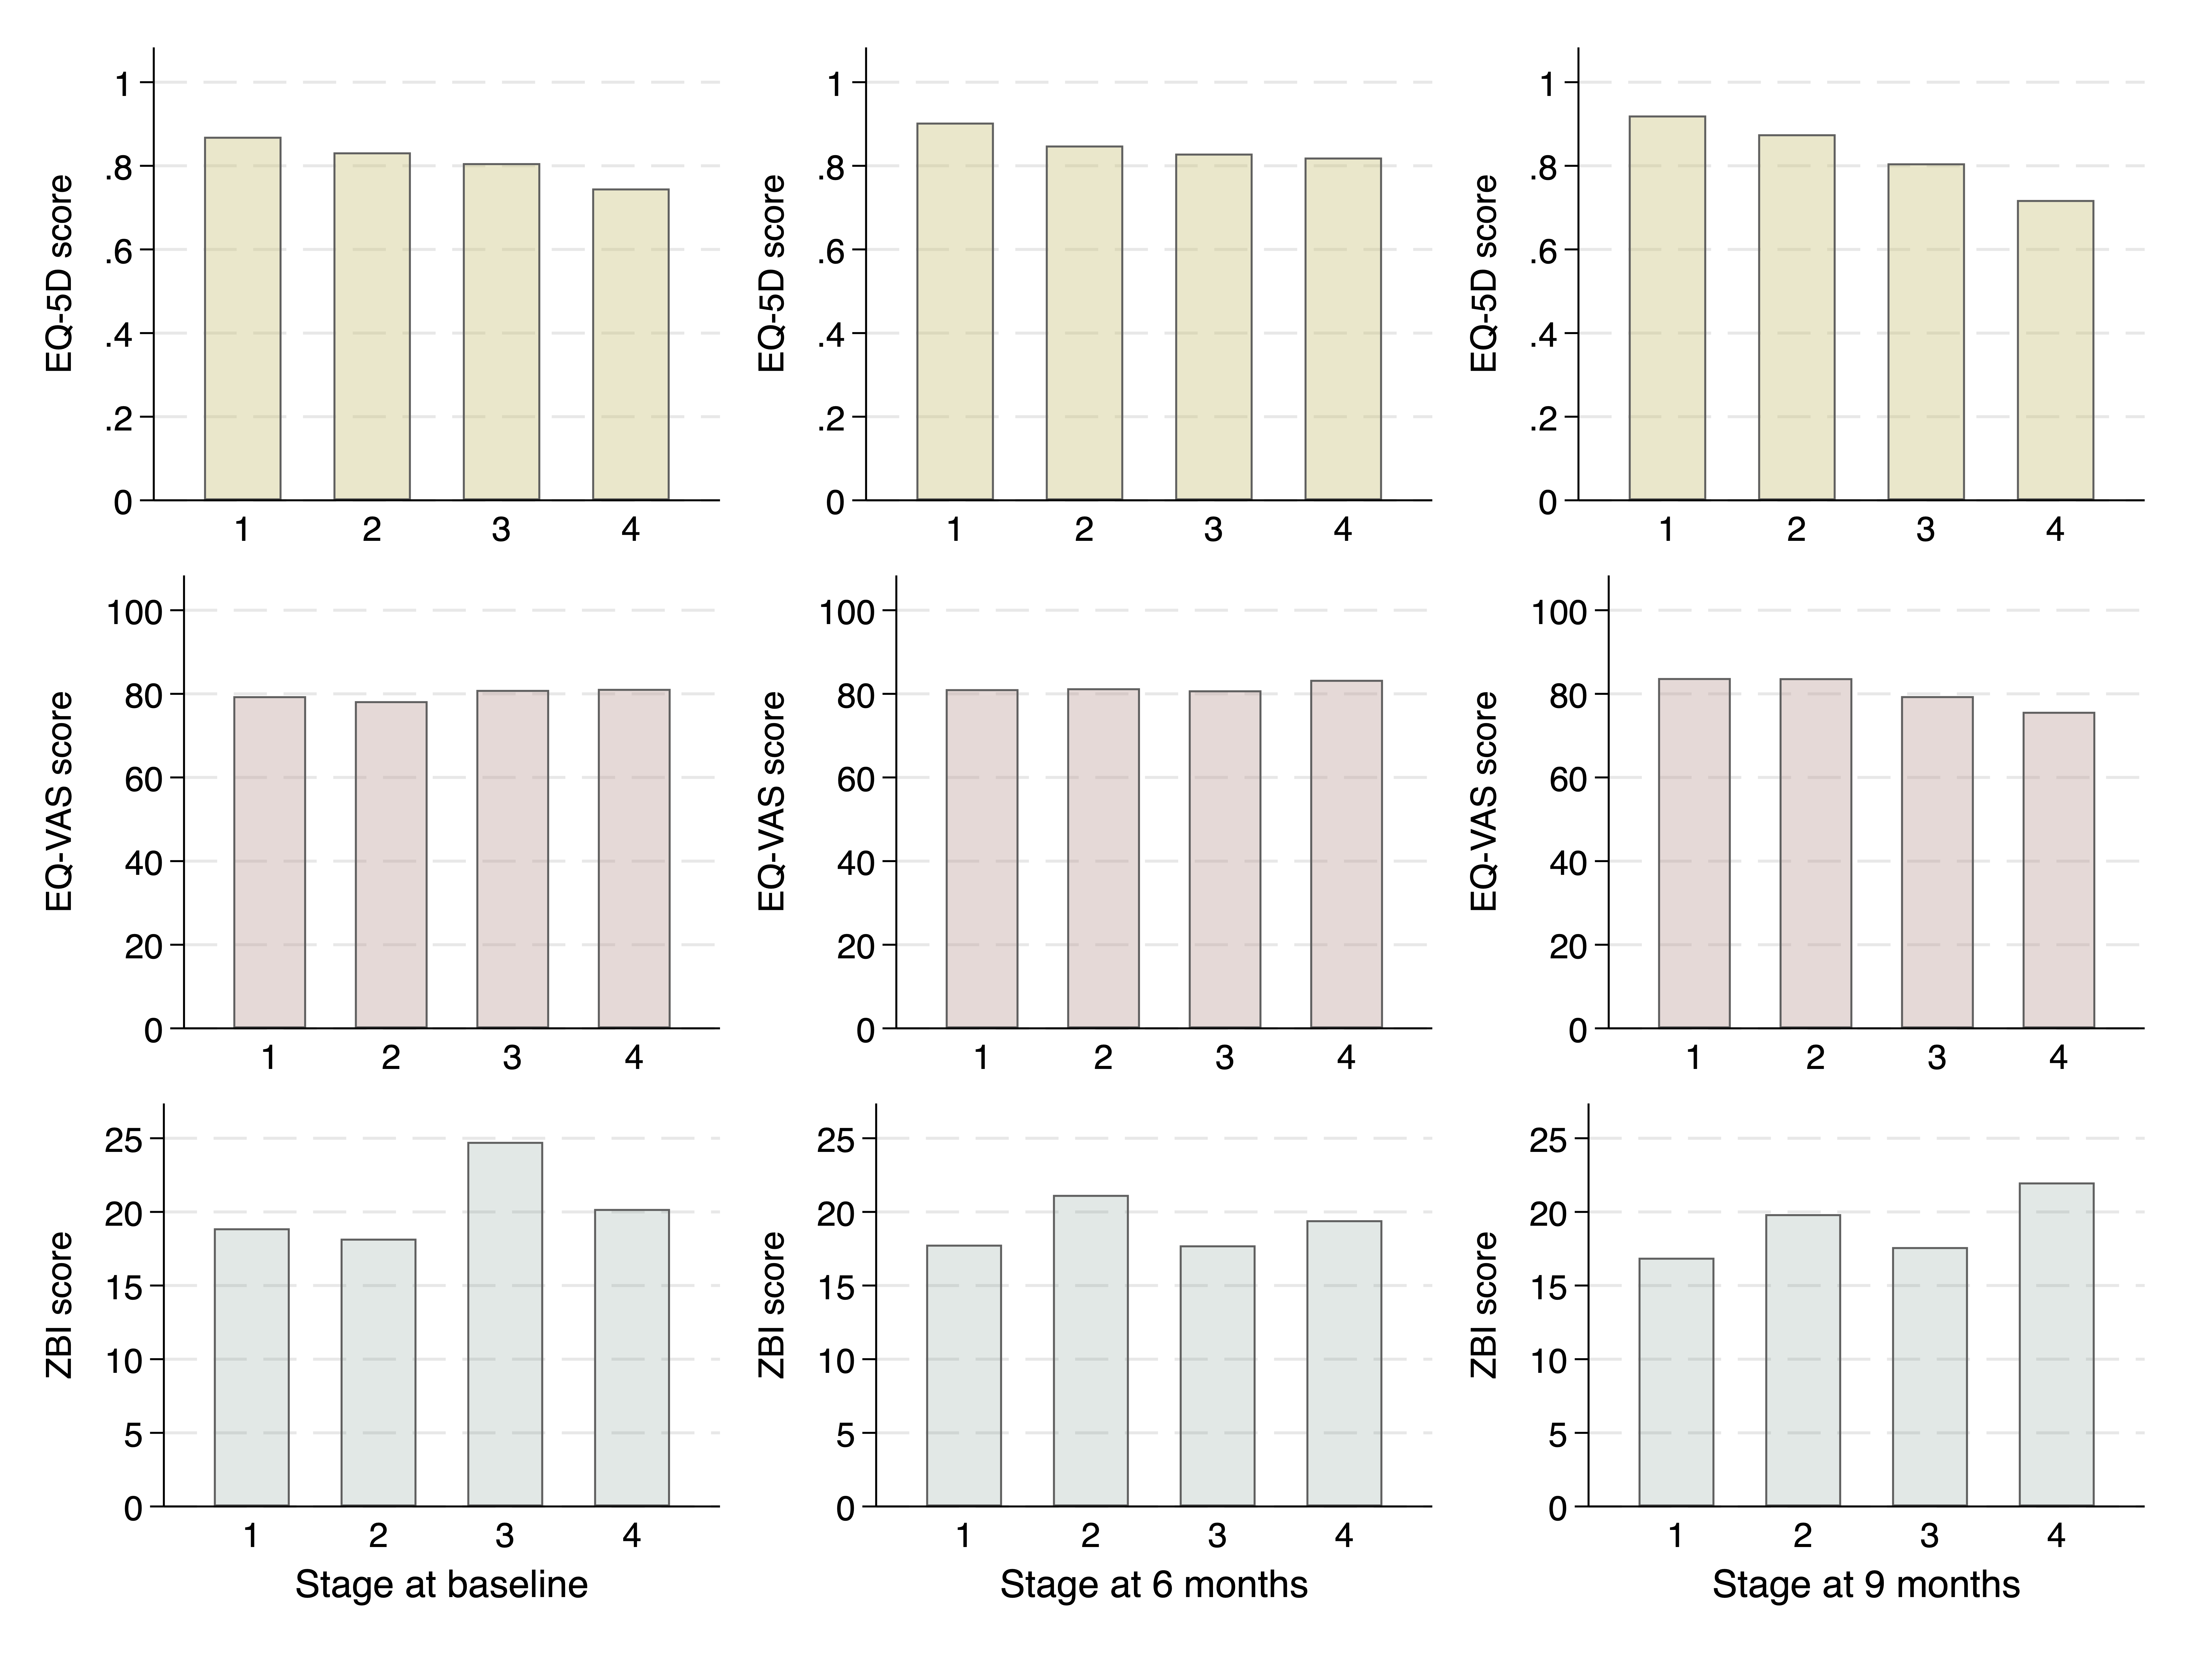
\includegraphics[width=1\linewidth]{figures/outcome-kings-stage.png}
    \caption{EQ-5D-5L utility scores, domain scores and scores by King’s stage}
    \label{fig:outcome-kings-stage}
    \caption*{\footnotesize \textit{Notes:} }
\end{figure}

\hspace{1em}
\begin{table}[H]
    \centering \singlespacing \small
    \caption{Pooled carer ZBI, EQ-VAS, and EQ-5D utility and domain scores by King’s stage}
    \begin{tabular}{|L{.33\linewidth}|R{.1\linewidth}|R{.1\linewidth}|R{.1\linewidth}|R{.1\linewidth}|R{.1\linewidth}|}
        \hline
        \PlainInput{tables/tab_outcomes_kings}
    \end{tabular}
    \label{tab_outcomes_kings}
    \caption*{\footnotesize 
                \textit{Notes:} Data from all caregivers at all time points (baseline, 6 months, and 9 months) have been pooled. Comparisons of outcomes between King’s stages use ANOVA. ZBI total score ranges from 0 to 88, with higher scores indicating greater burden. EQ-5D scores range from 0 to 1.0, with higher scores indicating better health-related quality of life. EQ-VAS scores range from 0 to 100, with higher scores indicate better health-related quality of life. EQ-5D domain scores range from 0 to 3, with higher scores indicating greater restriction by domain. \\
                ANOVA, analysis of variance; EQ-5D, EuroQol 5-dimension questionnaire; VAS, visual analog scale; ZBI, Zarit Burden Interview}
\end{table}


\subsection{Caregiver HRQoL}
%The EQ-5D-5L measured the HRQoL. The EQ-5D-5L index value (mean = 0.845/1, SD = 0.196) was higher than the EQ-VAS (mean = 71.16/100, SD = 20.47). Both values were slightly lower than in the general German population (EQ-VAS mean = 79.45/100, SD = 17.05 [71], EQ-5D-5L index value mean = 0.88/1, SD = 0.18) [72]. We found statistically significant differences of the EQ-VAS/EQ-5D-5L index value between the different BI groups (Figure 3a). Additionally, there was a slight positive correlation between the HRQoL (EQ-VAS/EQ-5D-5L index value) and the ALSFRS-R (rp = 0.278, p < 0.001/rp = 0.214, p = 0.001) and the BI (rp = 0.320, p < 0.001/rp = 0.258, p < 0.001) as well as the derived BI groups. Nonetheless, no statistically significant correlation between the EQ-VAS nor the EQ-5D-5L index value and the King’s Stages was found (Figure 3b). Overall, this examination displayed that there was a significant influence of the patient’s functional status on the decrease in CG’s HRQoL that was depicted by proxy- and self-reported functional scales but not the King’s Stages.

%The caregivers’ overall mean (SD) EQ-5D index score at baseline was 0.84 (0.20), and was 0.86 (0.18), 0.85 (0.19), and 0.82 (0.23) for the mild, moderate, and MS/S AD de- mentia groups, respectively (ANOVA P = 0.043), indicating a very slightly lower caregiver HRQoL for patients with MS/S AD dementia (Table 2). The overall caregiver mean (SD) EQ-5D VAS score at baseline was 75.1 (17.5), and by patient AD severity was 75.8 (16.6), 76.3 (16.5), and 72.9 (19.2) for the mild, moderate, and MS/S AD dementia groups, respectively (ANOVA P = 0.013). 

%\subsection{Caregiver HRQoL and burden over time}
%The mean (SD) change from baseline to 18 months was −0.02 (0.21) for the caregiver EQ-5D index score and −3.0 (18.5) for the caregiver EQ-5D VAS score. For both caregiver EQ-5D measures, the change from baseline to 18 months in the overall sample was not significant and did not differ significantly across the AD dementia severity groups (data not shown). Examination of the EQ-5D domain scores (Fig. 1) showed that very few caregivers had extreme problems (<5\% for any domain) and the levels of problems were similar at baseline and at 18 months. At both time points, more caregivers had some problems in the domains of pain/discomfort (baseline: 42.8\%; 18 months: 46.8\%) and anxiety/depression (baseline: 30.3\%; 18 months: 33.9\%) than in the other three domains.

\subsection{Relationship between ZBI and EQ-5D}
% SCH Figure 6 shows a correlation matrix of burden (ZBI score), depression (HADS-D score), anxiety (HADS-A score), HRQoL (EQ-VAS/EQ-5D-5L index value) and DOC. Several correlations between the parameters were observed. The statistically significant positive correlations between the ZBI and the HADS-D scores, as well as the HADS-A score and a negative correlation between the ZBI score and the EQ-VAS/EQ-5D-5L index value, confirmed the findings in the effect comparison between the highly and the lowly burdened CGs (see Section 3.5). Additionally, a statistically significant positive correlation was found between the HADS-D and the HADS-A scores, besides a negative correlation of both to the EQ-VAS/EQ-5D-5L index value, which indicated that depression, anxiety and lower HRQoL were interrelated. Nevertheless, this result has to be interpreted with caution as the overlap between the EQ-5D-5L domain anxiety/depression and the HADS might favor this effect. Furthermore, there was a statistically significant positive correlation between the DOC and the ZBI score, as well as to the HADS-D and HADS-A scores, compared to a negative correlation to the EQ-VAS/EQ-5D-5L index value. That indicated that an increased time spent with the patient went along with a higher caregiver burden, incidence of depression and anxiety and a lower HRQoL. Overall, due to existing correlations between all parameters, the caregiving strain appeared to result from complex interactions between different factors.

\subsubsection{ZBI and EQ-5D scores}
%Correlations were weak or very weak between EQ-5D (index and VAS scores) and ZBI or T-IADL at each time point and for the change scores (Table 3). For the ZBI, the 18-month change score correlation was −0.16 (95\% confidence interval, CI: −0.22, −0.09) for the EQ-5D VAS score and −0.09 (95\% CI: −0.15, −0.03) for the EQ- 5D index score. Caregiver T-IADL showed weak correl- ation with ZBI scores, and the 18-month change score correlation was 0.12 (95\% CI: 0.05, 0.18). However, there was no significant correlation between the 18- month change scores for T-IADL and the EQ-5D index score (Table 3).

\subsubsection{ZBI scores by EQ-5D domain}
%The mean ZBI total scores at baseline and at 18 months by EQ-5D domain showed that burden tended to be greater (higher mean ZBI total score) among caregivers with greater problem severity in each EQ-5D domain (data not shown). From baseline to 18 months, the HRQoL of the majority of caregivers (68–90\%) was stable in each EQ-5D domain, though some caregivers (3–14\%) showed better EQ-5D scores in some domains than at baseline. HRQoL worsened from baseline to 18 months in 7\% of caregivers within the self-care domain, 10\% within the mobility domain, 13\% in the usual activities domain, 17\% in anxiety/depression domain, and 18\% in the pain/discomfort domain (Fig. 2). %As evidenced by Fig. 2, which shows the mean change in ZBI total score by EQ-5D domain change category over 18 months, there was a trend for caregivers who experienced a worsening in EQ-5D domain score over 18 months to have the largest increases in ZBI total score (i.e., the greatest increase in caregiver burden).

\subsubsection{Factors influencing caregiver burden}
%As already shown above, the patient’s functional status had a clear influence on her/his caregiver’s burden. To provide a deeper analysis of further influencing factors on caregiver burden (ZBI score), multiple regression analysis was used (Table 3). The patient’s wheelchair dependency increased the ZBI score by 9.30 points. Additionally, a rise of 5.01 points was observed, if the patient needed permanent supervision. The main influence on the ZBI appeared to be the CG’s mental health impairment due to caregiving with an increase of 11.36 points. However, physical health impairment had no statistically significant impact on the ZBI score. Furthermore, patients’ age seemed to slightly lower the burden by −0.24 points for each increasing year. Neither the patient’s nor the CG’s gender had statistically significant impacts on the ZBI in the multivariate regression analysis.

\section{Discussion}
%%%%%%%%%%%%%%%%%%%%%%%%%%%%
%%% %%%
%%% Bibliography %%%

\clearpage
\newrefcontext[sorting=nyt]
\printbibliography


\end{document}
